\documentclass[12pt]{article}
\usepackage{hyperref} % 如果需要超链接功能
\usepackage{ctex} % 中文支持
\usepackage{tocloft}   % 用于控制目录格式(视情况看看是否需要这一行代码)
\usepackage{amsmath} % 数学公式支持
\usepackage{graphicx} % 图片支持
\usepackage{caption}  % 引入 caption 宏包

% https://liam.page/2014/09/08/latex-introduction/ 参考这个网站
\title{大四下学习笔记}
\author{杨昊}
\date{\today}
\begin{document}
% 生成标题
\maketitle
\thispagestyle{empty}  % 第一页不显示页码

\newpage
% 生成目录
\tableofcontents


\newpage

% 定义章节编号
\section{机器学习}


% 添加子目录(小节)
\subsection{理论}

\subsubsection{2025年2月25日:强化学习概念}
强化学习(Reinforcement Learning, RL)是一种机器学习方法,旨在通过与环境交互,使智能体(Agent)学习如何采取最优行动,以最大化某种累积奖励。它与监督学习和无监督学习不同,强调试错探索(Exploration-Exploitation)以及基于奖励信号的学习。
\begin{figure}[h]
    \centering
    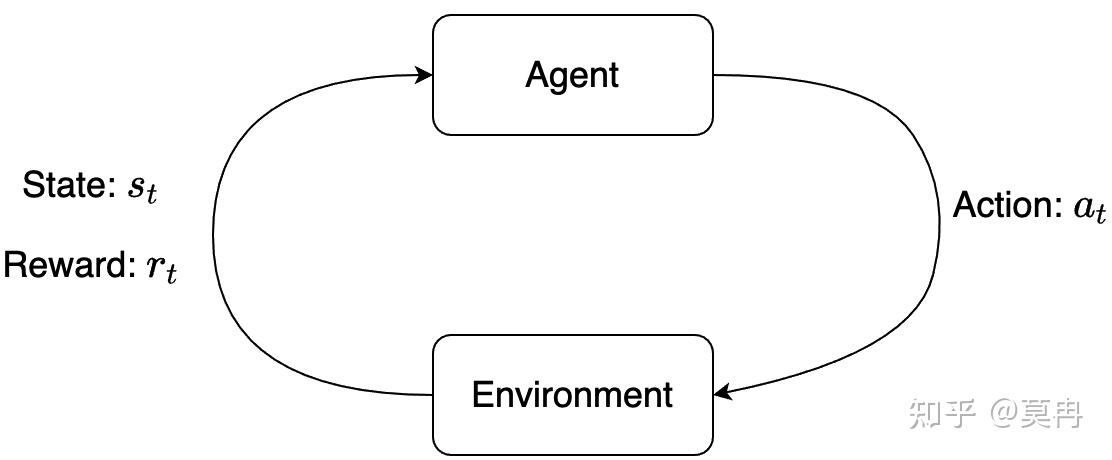
\includegraphics[width=0.7\textwidth]{./images/rlimage.jpeg}  % 图片文件名(包括路径)
\end{figure}

强化学习任务通常用马尔可夫决策过程来描述:机器处于环境$E$中,状态空间$X$,其中每个状态$x \in X$是机器感知到的环境的描述,机器能采取的动作构成了动作空间$A$,若某个动作$a \in A$作用在当前状态$x$上,则潜在的转移函数$P$将使得环境从当前状态按照某种概率转移到另一个状态,在转移到另一个状态的同时,环境会根据潜在的“奖赏”函数$R$反馈给机器一个奖赏。

机器要做的是通过在环境中不断地尝试而学得一个“策略”,根据这个“策略”在状态$x$下就能知道要执行得动作。

\textbf{在强化学习任务中,学习的目的就是要找到能使长期累积奖赏最大化的策略。}
\begin{quote}
    强化学习与监督学习来说,强化学习是没有人直接告诉机器在什么状态下应该做什么动作,只有等到最终结果揭晓,才能通过“反思”之前的动作是否正确来进行学习,因此,强化学习在某种意义上可看作具有“延迟标记信息”的监督学习问题。
\end{quote}
\subsubsection{2025年3月1日:评估模型的指标及正则化与交叉验证}
\noindent\makebox[\linewidth]{\hrulefill\quad 评估模型的指标 \quad\hrulefill}

对于分类模型,我们通常使用精度、召回率、F1 分数等指标来评估模型性能。

在分类任务中,混淆矩阵的每个元素表示真实值与模型预测值之间的关系。对于二分类问题,混淆矩阵通常是一个 2x2 的矩阵,包含以下四个元素:
\begin{quote}
    \begin{table}[h]
        \centering
        \begin{tabular}{|c|c|c|}  % 定义三列,所有列都居中对齐,使用竖线分隔

            \hline
            {真正例 TP} & 实际为正类的样本被模型预测为正类 \\
            \hline
            {假正例 FP} & 实际为反类的样本被模型预测为正类 \\
            \hline
            {真反例 TN} & 实际为反类的样本被模型预测为反类 \\
            \hline
            {假反例 FN} & 实际为正类的样本被模型预测为反类 \\
            \hline
        \end{tabular}
    \end{table}

\end{quote}
F1分数是精度和召回率的调和平均数。
\begin{itemize}
    \item 准确率(Accuracy):$A = \frac{TP+TN}{TP+TN+FP+FN}$
    \item 查准率、精度(Precision):$P = \frac{TP}{TP+FP}$
    \item 查全率、召回率(Recall):$R = \frac{TP}{TP+FN}$
    \item F1 分数:$F1 = \frac{2 \times P \times R}{P + R}$
\end{itemize}
ROC 曲线是一种用于评估分类模型性能的工具。它是通过不同的分类阈值(threshold)来绘制的,横轴是假正例率(False Positive Rate, FPR),纵轴是真正例率(True Positive Rate, TPR),即召回率(Recall)。
\begin{itemize}
    \item 假正例率(FPR):$FPR = \frac{FP}{FP+TN}$,表示实际为反类的样本被模型预测为正类的比例。
    \item 真正例率(TPR):$TPR = \frac{TP}{TP+FN}$,表示实际为正类的样本被模型预测为正类的比例。
\end{itemize}
AUC 是 ROC 曲线下的面积,表示模型在各种阈值下的表现。AUC 值的范围从 0 到 1,AUC 越接近 1,说明模型的性能越好。AUC 为 0.5 时,表示模型的分类效果相当于随机猜测,即没有任何分类能力;而 AUC 为 1 则表示模型的分类能力完美,能够完全区分正类和负类。

对于回归问题,常用的评估指标包括 均方误差(MSE) 和 决定系数(R²)。
\begin{itemize}
    \item 均方误差(MSE):$MSE = \frac{1}{n} \sum_{i=1}^{n} (y_i - \hat{y}_i)^2$
    \item 决定系数(R²):$R^2 = 1 - \frac{\sum_{i=1}^{n} (y_i - \hat{y}_i)^2}{\sum_{i=1}^{n} (y_i - \bar{y})^2}$,值越接近1,表示模型的拟合效果越好。
\end{itemize}

\noindent\makebox[\linewidth]{\hrulefill\quad 正则化与交叉验证 \quad\hrulefill}


正则化(Regularization) 是一种用于\textbf{防止模型过拟合的技术}。它是结构风险最小化策略的实现,是在经验风险上加一个正则化项或罚项。
\begin{quote}
    当模型复杂度过高(如参数过多或深度过深的神经网络)时,可能会很好地拟合训练数据,但在测试数据上表现较差,导致泛化能力下降。正则化通过限制模型的参数大小或稀疏化参数,减少对训练数据的过度拟合,使其在未见数据上的表现更稳定。
\end{quote}
正则化一般具有如下形式:
$$min_{f \in F} \frac{1}{N} \sum_{i=1}^{n} L(y_i, f(x_i)) + \lambda J(f)$$
其中,第一项是经验风险,第二项是正则化项,$\lambda > 0$为调整两者之间关系的系数。

常见的正则方式有
\begin{itemize}
    \item L1正则化(Lasso):$J(f) = ||f||_1 = \sum_{i=1}^{n} |w_i|$,即所有参数的绝对值之和。
          \begin{itemize}
              \item L1 正则化可以使得模型的参数稀疏化,即许多参数为 0,从而减少模型的复杂度。
              \item 适用于高位稀疏数据。
          \end{itemize}
    \item L2正则化(Ridge):$J(f) = ||f||_2^2 = \sum_{i=1}^{n} w_i^2$,即所有参数的平方和。
          \begin{itemize}
              \item L2 正则化不会使权重变为 0,而是让它们趋近于 0,使模型更平滑,减少对训练数据的敏感性,提高泛化能力。
              \item 适用于大部分回归问题。
          \end{itemize}
    \item Dropout:在训练过程中,随机将一部分神经元的输出置为 0,从而减少神经元之间的依赖关系,防止过拟合。
    \item 早停(Early Stopping): 在训练过程中,当验证集上的误差不再下降时,停止训练,防止模型过拟合。
\end{itemize}
在数据不充足时,为了选择好的模型,可以采用交叉验证(Cross Validation)的方法。
交叉验证的基本想法是重复地使用数据,把给定地数据进行切分,将切分地数据集组合为训练集与测试集,在此基础上反复地进行训练、测试以及模型选择。
\begin{itemize}
    \item 简单交叉验证:将数据集划分为训练集和测试集,只进行一次划分。
    \item K 折交叉验证:将数据集划分为 K 个大小相似的互斥子集,每次用 K-1 个子集的并集作为训练集,余下的子集作为测试集,共进行 K 次训练和测试。
    \item 留一交叉验证:K 折交叉验证的特例,K 等于数据集的大小。
\end{itemize}

\subsubsection{2025年3月2日:超参数调优及大模型基本概念}
\noindent\makebox[\linewidth]{\hrulefill\quad 超参数调优 \quad\hrulefill}

超参数调优是\textbf{机器学习模型训练过程中调整超参数以优化模型性能的过程}。
超参数是模型在训练前需要手动设定的参数,影响模型的学习能力和泛化能力。
常见超参数包括:学习率、正则化系数、决策树的最大深度、批量大小等。
合理的超参数选择可以显著提高模型的泛化能力,使其在新数据上的表现更优。
超参数调优的方法可分为手动调优和自动调优两大类。
\begin{itemize}
    \item 手动调参
          \begin{itemize}
              \item 手动调优依赖经验和试错法,适用于简单模型或对模型特性非常熟悉的情况。但手动调参的效率低,容易错过更优的参数组合。
          \end{itemize}
    \item 自动调参
          \begin{table}[h]
              \centering
              \begin{tabular}{|p{3cm}|p{5cm}|p{5cm}|} % 适当缩小列宽
                \hline
                \textbf{名字} & \textbf{原理} & \textbf{优缺点} \\ 
                \hline
                  网格调参(Grid Search) & 设定多个超参数的取值范围,遍历所有可能的组合进行训练,并选择最优结果。 & 可以找到全局最优;但是计算成本高 \\
                  \hline
                  随机搜索(Random Search) & 在设定的超参数范围内随机采样部分组合进行训练,而不是穷举所有组合。 & 比网格搜索计算量小;但是不能保证找到最优解 \\
                  \hline
                  贝叶斯优化(Bayesian Optimization) & 使用概率模型(如高斯过程)建模超参数对目标函数(如验证集误差)的影响,并通过探索和利用策略选择最优超参数。 & 比随机搜索效率更高效;但是计算成本极高 \\
                  \hline
              \end{tabular}
          \end{table}

\end{itemize}

\noindent\makebox[\linewidth]{\hrulefill\quad 大模型基本概念 \quad\hrulefill}
大模型(Large Model)是指具有大规模参数和复杂计算结构的机器学习模型。

大语言模型(Large Language Model):通常是\textbf{具有大规模参数和计算能力的自然语言处理模型},例如ChatGPT、deepseek。这些模型可以通过大量的数据和参数进行训练,以生成人类类似的文本或回答自然语言的问题。

生成式AI(Generative AI)是指能够生成文字、图片、音频、视频等多种内容的人工智能系统。\textbf{大语言模型(LLM)是生成式 AI 的一种,但生成式 AI 不仅限于语言,还包括图像、视频、音乐等。}

多模态AI(Multimodal AI)进一步扩展了生成式 AI 的能力,使其\textbf{能够处理文本、图像、音频、视频等多种数据类型。}

通用人工智能(AGI:Artificial General Intelligence)指的是能够像人类一样理解、学习和执行多种任务的智能系统。

\begin{figure}[h]
    \centering
    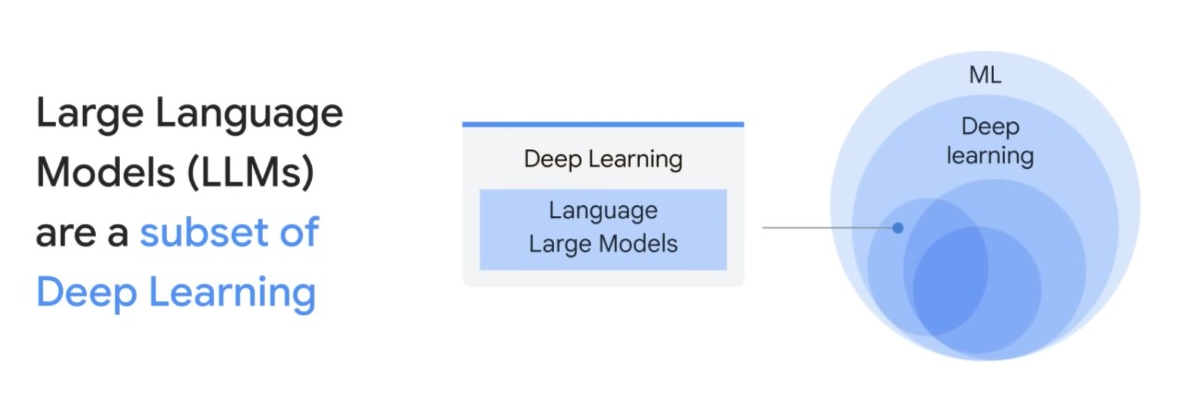
\includegraphics[width=0.7\textwidth]{./images/llmML.png}
    \caption*{大语言模型机器学习的联系}
\end{figure}
大模型的参数很大,例如:LLaMA 2: 7B、13B、65B。\textbf{这里的B是bilion(十亿)的意思},表示LLaMA2有70亿、130亿、650亿个参数。

在使用大语言模型时,总会看到token一词,调用大模型api是根据token的使用数进行付费。\textbf{大模型的token 并不等同于单词,一个token可能是一个单词、一部分单词,或者一个标点符号。}

\subsubsection{2025年3月3日:逻辑斯蒂回归数学推导}
逻辑斯蒂分布的分布函数:
$$F(x) = P(X \le x) = \frac{1}{1 + e^{-(x - \mu) / \gamma}}$$
其中,$\mu$为位置参数,$\gamma$为尺度参数。该函数的形状为 S 型曲线,常用于二分类问题。

二项逻辑斯蒂回归模型由条件概率分布$P(Y|X)$表示,其中随机变量$Y$取值为 0 或 1,随机变量$X$为实数。
\begin{align}
    P(Y=1|X) &= \frac{ e^{w \cdot x + b} }{1 + e^{w \cdot X + b}} \\
    P(Y=0|X) &= 1 - P(Y=1|X)
\end{align}

几率是指事件发生的概率与不发生的概率之比,即$logit(p) = \frac{p}{1-p}$。逻辑斯蒂回归模型的几率为:
$$
log \frac{P(Y=1|X)}{1 - P(Y=1|X)} = w \cdot x + b
$$
在逻辑斯蒂回归模型中,输出$Y=1$的对数几率是输入$x$的线性函数。

之后可以采用极大似然法估计模型参数。
$$
P(Y=1|x) = \pi(x), P(Y=0|x) = 1 - \pi(x)
$$

那么似然函数为:
$$
\sum_{i=1}^{N} \pi(x_i)^{y_i} (1 - \pi(x_i))^{1-y_i}
$$

对数似然函数为:
$$
L(w) = \sum_{i=1}^{N} y_i log \pi(x_i) + (1 - y_i) log (1 - \pi(x_i))
$$

对$L(w)$求导,得到$w$的估计值。
问题转换为以对数似然函数为目标函数的最优化问题。
学到的逻辑斯蒂回归模型为:
\begin{align*}
    P(Y=1|X) &= \frac{ e^{\hat{w} \cdot x + b} }{1 + e^{\hat{w} \cdot X + b}} \\
    P(Y=0|X) &= 1 - P(Y=1|X)
\end{align*}

推广为多项逻辑斯蒂回归模型,用于多分类问题:
$$
P(Y=k|x) = \frac {e^{w_k \cdot x + b_k}}{\sum_{k=1}^{K} e^{w_k \cdot x + b_k}} , k = 1,2,...,K
$$

\subsubsection{2025年3月6日:Karpathy的大语言模型介绍}
2025年3月4日:Karpathy的大语言模型介绍超链接:\href{https://www.bilibili.com/video/BV16cNEeXEer/?spm_id_from=333.337.search-card.all.click&vd_source=13dfbe5ed2deada83969fafa995ccff6}{B站视频链接}。

大模型流程分为:预训练(pre-training)和后训练(post-training)两个阶段。预训练是为了让模型学习到大量的数据,提高模型的泛化能力;后训练是为了让模型适应特定任务,提高模型的性能。

预训练阶段步骤如下:
\begin{enumerate}
    \item 下载和处理互联网数据
    \item 标记化和分词:通过分词器将一维文本序列重新表示为一个token序列的过程。(可以使用https://tiktokenizer.vercel.app/网站查看token)
    \item 神经网络训练:根据数据集实际发生的统计数据及其概率变得与这些token在数据中如何相互跟随的统计模式一致。\textbf{神经网络参数中的知识是模糊的记忆}。
    \item 推理:使用预训练的模型生成文本。
\end{enumerate}
此时就得到了一个\textbf{基础模型},可以用于生成文本。它是一个token级互联网文档模拟器,由于是随机生成的,所以每次运行都会得到不一样的内容。

后训练阶段包含\textbf{监督微调SFT}和\textbf{强化学习RL}。监督微调是通过示例文本对模型进行训练,强化学习是通过奖励函数对模型进行训练(练习问题)。
监督微调创建对话数据,用对话协议进行标记化。强化学习是通过奖励函数对模型进行训练,不依赖人类标注、猜测和检查。

\begin{figure}[h]
    \centering
    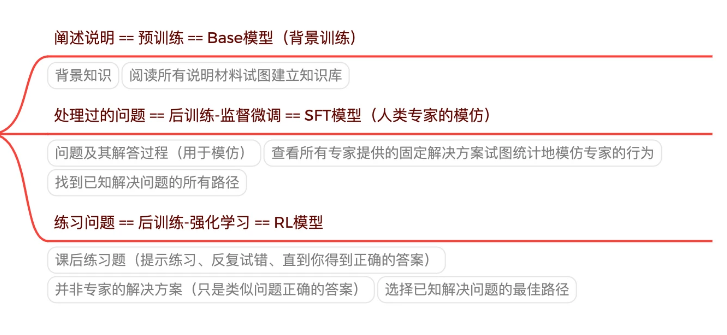
\includegraphics[width=0.7\textwidth]{./images/karpathyllm.png}
\end{figure}


\textbf{幻觉}是模型可能出现的一种问题,表现为捏造内容,生成虚假或不存在的信息。
同时,模型在处理记忆时,可能会出现模糊记忆,即记忆内容不清晰、不准确,与工作记忆形成对比。
工作记忆是指短期记忆,用于处理和存储当前任务所需的信息。同时,模型对自身的了解和认知,即自我知识,也存在一定的局限性。

在模型的局限性方面,模型需要通过token来思考,这在一定程度上限制了其处理信息的方式。
模型在计数方面存在困难,不擅长拼写,并且由于是基于token级的模型,导致其无法看到字符。

想要模型对专有信息进行理解,增强模型在特定行业领域的知识,使用\textbf{SFT}。有监督微调(SFT,Supervised Fine-Tuning)通过提供人工标注的数据,进一步训练预训练模型,让模型能够更加精确地处理特定领域地任务。
除了”有监督微调”,还有“无监督微调”和“自监督微调”,当提到“微调”时,通常指的是“有监督微调”。


提高个性化和互动性强的服务,使用\textbf{RLHF}。强化学习(RLHF,Reinforcement Learning from Human Feedback)分为DPO(Direct Preference Optimization)和PPO(Proximal Policy Optimization)两种方法,通过人类反馈来训练模型,提高模型的性能。
\begin{itemize}
    \item DPO:通过\textbf{人类对比选择}直接优化生成模型,使其产生更符合用户需求地结果。
    \item PPO:通过\textbf{奖励信号}来渐进式调整模型地行为策略。
\end{itemize}

提高模型对专有信息的理解,增强模型在特定行业领域的知识,获取和生成最新的、实时的信息,使用\textbf{RAG}。
检索增强生成(RAG,Retrieval-Augmented Generation)将外部信息检索与文本生成结合,帮助模型在生成答案时,实时获取外部信息和最新信息。

微调适合有充分地数据,能够直接提示模型地固有能力,无需依赖外部检索;RAG适合只有非常少地数据,动态更新的数据,每次回答问题前需要耗时检索知识库,回答质量依赖于检索的质量。
少量私有数据最好微调和RAG都做;会动态更新的知识使用RAG;大量垂直领域的知识用微调。

预训练模型(基座模型)指的是已经在大量数据上训练过的模型,也就是我们微调前需要预先下载的开源模型。它具备了较为通用的知识和能力,能够解决一些常见的任务,开源在此基础上进行进一步的微调,以适应特定的任务或领域。

微调算法分为全参数微调和部分参数微调。全参数微调对整个预训练模型进行微调,会更新所有参数,通常可以达到最佳性能,但是计算资源大,可能过拟合;部分参数微调只更新模型的部分参数,检索了计算成本,但是可能无法达到最佳性能。

LoRA是著名的部分参数微调算法,通过低秩矩阵分解的方式来进行部分参数微调。矩阵的秩是指矩阵中线性无关的行或列额最大数量,反应矩阵所包含的有效信息量。
$$
h = W_0x + \triangle Wx = W_0x + BAx
$$
其中,$h$是模型输出,$W_0$是预训练模型的参数,,是一个全秩矩阵;$x$是模型输入;
$\triangle W_0$是微调后元素权重的变化量,,也是一个全秩矩阵,大小和$W_0$相同;$BA$是两个低秩矩阵,它们的乘积表示对原始权重的微调变化量
$\triangle W_0$。

$W_0x + \triangle Wx$是全参数的输出;$W_0x + BAx$是部分参数的输出。LoRA训练结束后通常需要进行权重合并。
\subsection{实践}


dff
\section{有限元分析}

\end{document}
